\documentclass[
    landscape,      % landscape or portrait
    paperwidth = 1200mm,
    paperheight = 900mm,
    fontscale = 0.34,
    margin = 1.7cm,
]{baposter}
\definecolor{lightblue}{rgb}{0.145,0.6666,1}
\usepackage{times}
\usepackage{tikz}
\usepackage{floatrow}
\usepackage{hyperref}

\begin{document}

\begin{poster}{
    % poster environment options
    grid = false,            % true or false
    columns = 3,
    colspacing = 0.6em,
    bgColorOne = white,
    bgColorTwo = white,
    background = plain,     % plain, shade-lr, shade-tb, user, none
    eyecatcher = true,      % eye catcher on the left of the title page
    % posterbox environment options
    borderColor = blue,
    headerColorOne = black,
    headerColorTwo = lightblue,
    headerFontColor = white,
    textborder = roundedleft,   % none, bars, coils, triangles, rectangle
                                % rounded, faded, roundedsmall, roundedleft
                                % roundedright
    headerborder = closed,      % none, closed, open
    headershape = roundedright, % rectangle, small-rounded, roundedleft,
                                % roundedright, rounded
    headershade = shadelr,      % plain, shadelr, shadetb, shade-tb-inverse
    boxshade = none,            % plain, shade-lr, shade-tb, none
    headerfont = \Large\bf\textsc,
    linewidth = 0.1 em,}
{
\includegraphics[height=9em]{USTC_logo_blue.jpg}}
{\huge{3D Crust and Uppermost Mantle Structure beneath Tian Shan Region from ambient noise and earthquake surface waves}}
{
    \vspace{0.3em}
    Xiao Xiao$^1$ (\textcolor{blue}{xiaox17@mail.ustc.edu.cn}),
    Lianxing Wen$^{2,1}$ \\
    \vspace{0.3em}
    1. Laboratory of Seismology and Physics of Earth's Interior, University of Science and Technology of China  \\
    2. Department of Geosciences, State University of New York at Stony Brook  \\
}
{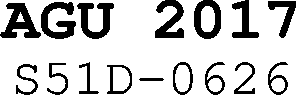
\includegraphics[height=5em]{2017_AGU_ID}}
\vspace{0.4cm}

\begin{posterbox}[column=0, row=0]{1. Introduction}
\setlength{\parskip}{3pt}
As a typical active intracontinental mountain range in Central Asia, Tian
Shan Mt serves as the prototype in studying geodynamic processes and mechanism
of intracontinental mountain building.
We study 3D crust and the uppermost mantle structure beneath Tian Shan and close region
using ambient noise and earthquake surface waves.
\end{posterbox}

\begin{posterbox}[column=0, below=auto]{2. Data and Methods}
\setlength{\parskip}{3pt}
My data set contains 60 brand-band seismic stations mainly
locating at foot of Tian Shan mountain and joint area.
Several stations, situating at the sounthern foot of Altai Mt. and northern foot of Kunlun Mt.,
provide critical ray path coverage of Junggar amd Tarim basins.Our dataset includes vertical
component continuous record from 2015 to 2016 and teleseismic waveforms,
whose magnitudes are over 5.5, focal depths are shallower than 200 km and happened during
2013 and 2016.

 Firstly, we measure group velocity diospersion curve of fundamental-mode Rayleigh wave in the period of 3 to 45 s using
 a frequency-time analysis method from two-year stacked Empirical Green's Function (EGF).
 Secondly, we collect surface wave data from tele-seismic events and measure group velocities of the fundamental-mode
 of Rayleigh wave in the period of 25 to 55 s using a two-station method.
 Finally, we combine the group velocity dispersion curves measured from ambient noise and earthquake surface waves,
 obtain lateral isotropic group velocity maps at different periods based on tomography and invert a 3D Vsv model of crust
 and uppermost mantle down to about 70 km using a Monte Carlo Inversion method.


\begin{center}
  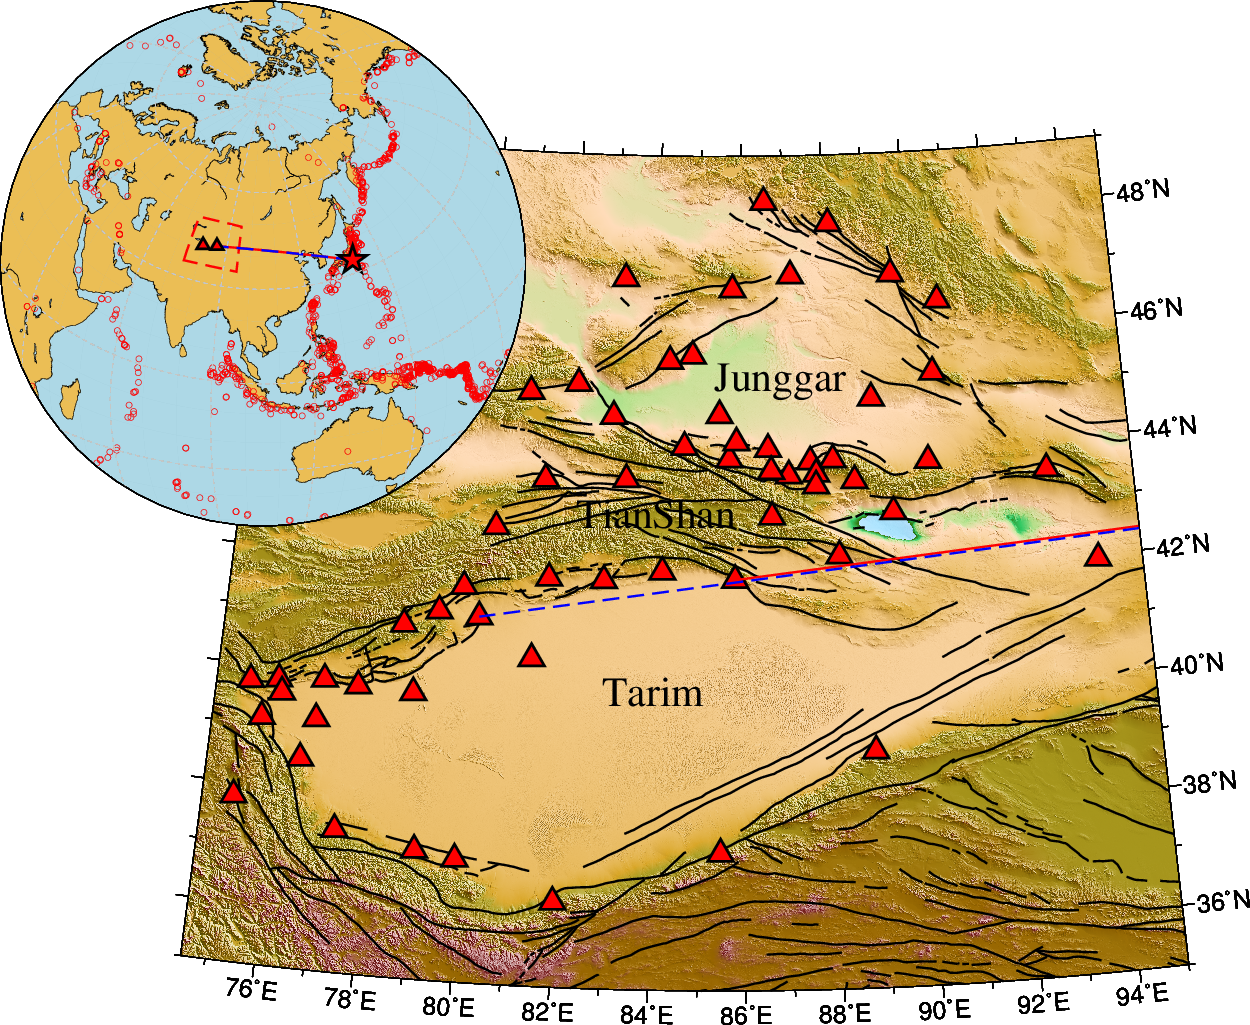
\includegraphics[width=.6\textwidth]{XJ}
\end{center}

\begin{center}


\begin{minipage}{0.9\textwidth}
\small
\textbf{Fig. 1.}
\itshape
Map of research area. Red triangles represent broad-band seismic stations
in Tianshan area used in this study. Solid black thick lines show the faults.
The insert (top left) depicts telsesimic distribution. Red circles represent
epicenter of teleseismic used in this study, which happened from 2013 to 2016.
Dashed red square is study area. Two triangles represent two stations named as
AKS and KOL, which are in common line with this star-labelled earthquake.
\end{minipage}
\end{center}

\begin{center}
\begin{minipage}{0.6\textwidth}
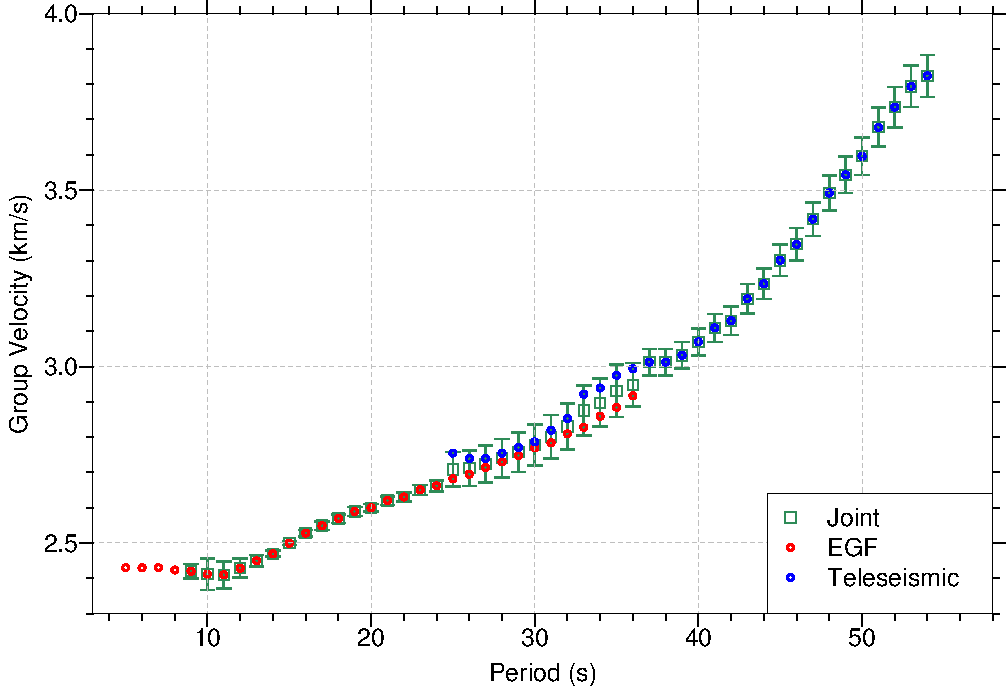
\includegraphics[width=\textwidth]{JointDisp}
\end{minipage}
\hspace{0.1cm}
\begin{minipage}{0.35\textwidth}
\footnotesize
\textbf{Fig. 2.}
\itshape
Demos of combination of group velocity dispersion curves between two stations, AKS and KOL.
Red circles denote dispersion points measured from EGF while blue circles represent those measured from teleseismic.
Limegreen squares give combined dispersion curve. At overlap periods, green squares are weight average of blue and red circles
, in which weights are inverse of their error which summation of their errors gives error of combined dispersion curve.
\end{minipage}
\end{center}


\end{posterbox}

\begin{posterbox}[column=1]{3. 2D Group velocity Maps}
In this section, we present inverted 2D group velocity maps.
\begin{center}
\begin{minipage}{0.62\textwidth}
\begin{tikzpicture}[nodes={inner sep=0}]
\node (a) {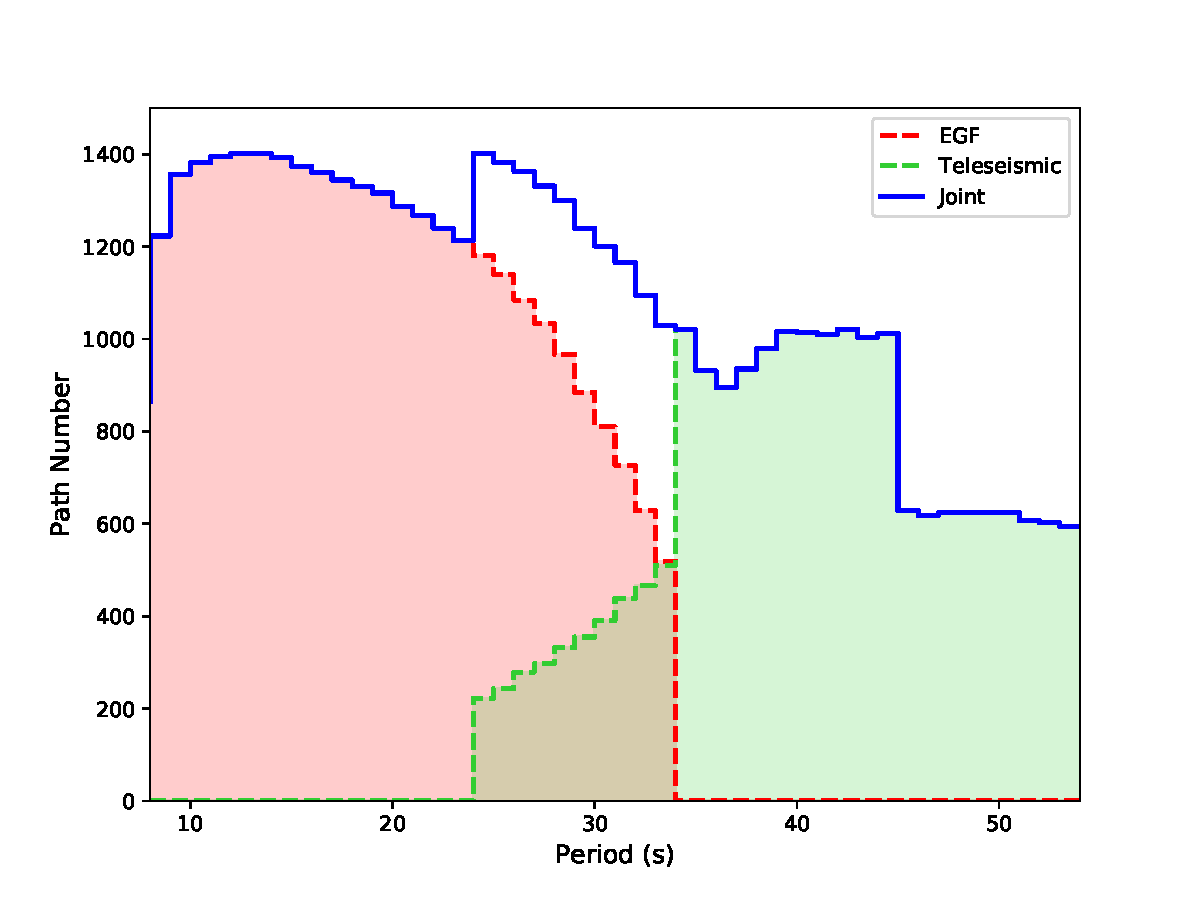
\includegraphics[width=\textwidth]{Pathnum}};
\end{tikzpicture}
\end{minipage}
\begin{minipage}{0.35\textwidth}
\footnotesize
\textbf{Fig. 3.}
\itshape
Dispersion curve numbers used for tomography, variate with period. The Dashed
limegreen line and corresponding limegreen area shows number of used dispersion
curves measured from teleseismic with two-station method while Dashed
red line and area denote number of those measured from EGF at each period. The
solid blue line indicates numbers of all used dispersion curves which are summation of
above two.
\end{minipage}
\end{center}

The PKiKP-PcP differential travel time residuals exhibits
large spatial variations from -1.0 s to 1.0 s in a horizontal distance of
about $5^\circ$ (Fig. 2).




The PKiKP-PcP differential travel time residuals have a positive correlation
with PKiKP travel time residuals (Fig. 3a), while no correlation is found with PcP
travel time residuals (Fig. 3b), implying that the large variations of PKiKP-PcP
residuals mainly come from PKiKP phases. A typical ULVZ model of a 10\%
decrease in P wave velocity over a 15 km layer near the PKiKP entrant or
exit points at the CMB, gives a travel time pertubation of about 0.12 s,
which is not quite large enough to account for the observed variation of 1.0 s.
Thus, the observed PKiKP-PcP differential travel time residuals may indicate
a ICB topographic change of 5 km.

\begin{center}
%\includegraphics[width=0.95\textwidth]{Mexico_Vesus}
\begin{minipage}{0.9\textwidth}
\footnotesize
\vspace{0.2em}
\textbf{Fig. 3.}
\itshape
Relationship among PKiKP-PcP differential travel time residuals, PKiKP
travel time residuals and PcP travel time residuals. Events are coded
using different colors.
\end{minipage}
\end{center}

\vspace{-0.15cm}
The binned PKiKP/PcP amplitude ratios exhibit much larger values than
predictions of different ICB models (Fig. 4) and spatial variations (Fig. 5).
\begin{center}
\begin{minipage}{0.50\textwidth}
%\includegraphics[width=\textwidth]{Mexico_ratio_gcarc}
\begin{minipage}{0.98\textwidth}
\vspace{0.1cm}
\footnotesize
\textbf{Fig. 4.}
\itshape
Observed PKiKP/PcP amplitude ratios (dots) as a function of epicentral distance,
with predictions (lines) of different P wave speed (a) and density (b) constrasts
across the ICB. The red squares represent average amplitude ratios of each bins, and
the error bar represnt standard deviations.
\end{minipage}
\end{minipage}
\hspace{0.2cm}
\begin{minipage}{0.45\textwidth}
%\includegraphics[width=\textwidth]{Mexico_region_ratio}
\begin{minipage}{0.98\textwidth}
\vspace{0.3cm}
\footnotesize
\textbf{Fig. 5.}
\itshape
Binned PKiKP/PcP amplitude ratio residuals, defined as the ratio between
observed and predicted PKiKP/PcP amplitude ratios. $1^\circ$ geographical
bins with the bin centers shift by $1^\circ$ in latitude and longtitude are used.
The ratio residuals are plotted at the mean PKiKP reflection locations in each bins.
\end{minipage}
\end{minipage}
\end{center}
\end{posterbox}

\begin{posterbox}[column=2 ]{4. ICB Beneath the Bearing Sea}
In this section, we present seismic observations which sample the ICB region beneath
Bearing Sea (Fig. 1b). The small variations of the PKiKP-PcP differential
travel time residuals indicate a flat ICB in this region (Fig. 6).


The linear relationship between PKiKP and PcP travel time residuals (Fig. 7)
indicates that most variations in PKiKP and PcP travel time residuals
originate from shallow Earth's hetergeneity, which can be effectively
eliminated by using PKiKP-PcP differential travel time residuals.
\begin{center}
\begin{tikzpicture}[nodes={inner sep=0}]
%\node (a) {\includegraphics[width=0.8\textwidth]{Bearing_Vesus.pdf}};
\end{tikzpicture}
\begin{minipage}{0.9\textwidth}
\footnotesize
\vspace{0.5em}
\textbf{Fig. 7.}
\itshape
Relationship among PKiKP-PcP differential travel time residuals, PKiKP
travel time residuals and PcP travel time residuals.
\end{minipage}
\end{center}

The stacked PKiKP and PcP waveforms show similar waveforms (Fig. 8), indicating a sharp
interface at both the CMB and ICB. The PKiKP/PcP amplitude ratios exhibit
large scattering on single records.
The PKiKP/PcP amplitde ratios binned by epicentral distance,
exhibit much larger amplitude ratios than predictions of different ICB models (Fig. 9).

\begin{center}
\begin{minipage}{0.32\textwidth}
%\includegraphics[width=\textwidth]{Bearing_stack}
\begin{minipage}{0.98\textwidth}
\footnotesize
\textbf{Fig. 8.}
\itshape
Comparisons of stacked PKiKP (blue) and PcP (black) waveforms in each
geographical bins. The locations of the bins center and the number of traces
used in each stacking are labeled at the right of each traces.
\end{minipage}
\end{minipage}
\hspace{0.4cm}
\begin{minipage}{0.52\textwidth}
%\includegraphics[width=\textwidth]{Bearing_ratio_gcarc}
\begin{minipage}{0.98\textwidth}
\footnotesize
\textbf{Fig. 9.}
\itshape
Observed PKiKP/PcP amplitude ratios (dots) as a function of epicentral distance,
with predictions (lines) of different P wave speed (a) and density (b) constrasts
across the ICB. The red squares represent average amplitude ratios in each bins, and
the error bar represnt standard deviations.
\end{minipage}
\end{minipage}
\end{center}
\end{posterbox}

\begin{posterbox}[column=2, below=auto]{5. Conclusions}
We collect a large dataset of high-quality PKiKP waveforms, and use
PKiKP-PcP differential travel time residuals, PKiKP/PcP amplitude ratios,
and PKiKP-PcP waveform differences to constrain ICB properties.
Based on the observations, the ICB beneath Bearing Sea has a sharp and flat
boundary, and the ICB beneath Mexico may have a bumpy ICB with a topographic
height change of 5 km. PKiKP/PcP amplitude ratios are much larger than predictions,
implying possible other factors which affects the amplitude ratios.
\end{posterbox}

\end{poster}
\end{document}
